\documentclass[a4paper,12pt,normaltoc,capchap]{abnt}
\usepackage{abnt-UEPG}
\usepackage[top=3cm,bottom=2cm,left=3cm,right=2cm]{geometry}
\usepackage[utf8]{inputenc}
\usepackage[brazil]{babel}
\usepackage[T1]{fontenc}
%\usepackage{hyperref}
\usepackage{amssymb}
\usepackage{amsmath}
\usepackage{paralist}
\usepackage{graphicx}
\usepackage{subfigure}
\usepackage{setspace}
\usepackage{fancyhdr}
\usepackage{lscape}
\usepackage{longtable}
\usepackage{fancyvrb}
\usepackage[alf,abnt-etal-text=it,bibjustif]{abntcite}
\usepackage{listings}
\usepackage{fancychap}
\usepackage{makecell}
\usepackage{multirow}
\usepackage{tipa}
\usepackage{array,multirow,graphicx}
\usepackage[table,xcdraw]{xcolor}
\renewcommand{\lstlistingname}{Código} % definição visual dos códigos fonte

%%%%%%%% lista de quadros
\usepackage{trivfloat}
\trivfloat{quadro}
\floatstyle{plaintop} % Forçar posição da legenda para o topo
\restylefloat{quadro} % Forçar posição da legenda para o topo
\addto\captionsbrazil{%
\renewcommand{\listquadroname}{Lista de Quadros}}


\lstset{language=Java, basicstyle=\footnotesize, numbers=left, frame=tb, breaklines=true, basicstyle=\footnotesize}

%------------------------------------------------------------------------------
% Dicionário de hifenização em português
%------------------------------------------------------------------------------

\hyphenation{pro-ces-sa-men-to}
\hyphenation{a-pre-sen-ta-da}
\hyphenation{pro-gra-ma}
%------------------------------------------------------------------------------
% Configurações da dissertação
%------------------------------------------------------------------------------


\instituicao{UNIVERSIDADE ESTADUAL DE PONTA GROSSA\\
PRÓ-REITORIA DE PESQUISA E PÓS-GRADUAÇÃO\\
PROGRAMA DE PÓS-GRADUAÇÃO EM CIÊNCIAS BIOMÉDICAS\\ }

\autor{AUTOR AUTOR AUTOR}

\titulo{TITURLO TITULO}

\comentario{Trabalho de Conclusão de Curso apresentado para a obtenção do título de Bacharel em Engenharia de Software pela Universidade Estadual de Ponta Grossa. \\ \\Orientadora: Prof Dra. D \\ Coorientador: Prof MSc. M}

\local{Ponta Grossa}

\data{2017}

%------------------------------------------------------------------------------
% Início do documento 
%------------------------------------------------------------------------------

\begin{document}

\capa

\folhaderosto
%

\

\vfill

\begin{flushright}
\hfill \textit{É bom sentir-se melhor, mas é melhor sentir-se bem.\\ 
(Maxime Dougados)}
\end{flushright}

\vspace*{1cm}

\clearpage
\

\vfill

\begin{flushright}
\hfill \textit{Dedico este trabalho aos meus queridos pais,\\ que por amor fizeram de tudo por mim. }
\end{flushright}

\vspace*{1cm}

\clearpage
\chapter*{Agradecimentos}
À Deus, que esteve presente em todos os momentos, me guiou com sua luz divina, ouviu minhas preces e me fortaleceu. A Ti, meu Deus, toda honra e toda glória eternamente.
\begin{resumo}

{\noindent A Qualidade de Vida (QV) é definida pela Organização Mundial de Saúde (OMS) como algo subjetivo e de natureza multidimensional, visto que vários fatores a influenciam. Estudos recentes demonstram que a condição bucal pode atuar como um fator modificador para a QV de indivíduos portadores de doenças crônicas. Objetivo: Avaliar o impacto da saúde bucal sobre a qualidade de vida de pacientes com Doença Renal Crônica (DRC) em Hemodiálise (HD). Métodos: Trata-se de um estudo caso controle de caráter observacional e transversal, com aplicação de questionários estruturados para 100 pacientes com DRC em hemodiálise (Grupo DRC) pareados com 100 pacientes controles (Grupo Controle). Os dados demográficos e de escolaridade foram obtidos em formulário elaborado especificamente para a pesquisa. A classificação da condição socioeconômica seguiu os critérios da Associação Brasileira de Empresas de Pesquisas. A qualidade de vida, bem como, o impacto da saúde bucal sobre a QV foi avaliado através dos seguintes questionários respectivamente: 1) “\textit{The Short Form Health Survey} (SF-36)” e 2) “\textit{Oral Health Impact Profile-14} (OHIP-14)”. Resultados: A média total do OHIP-14 para o grupo controle foi de 6,06 ($\pm$ 7,44) e de 4,67 ($\pm$ 6,52) para o grupo DRC. Ao comparar os valores internos do OHIP-14 entre os grupos controle e DRC, não foi observado diferença estatisticamente significativa entre os grupos. Em relação a qualidade de vida geral avaliada pelo SF-36, o grupo DRC obteve os piores scores para os domínios “capacidade funcional” e “limitação por aspectos físicos”. Em relação a QV geral no grupo controle, este grupo apresentou pior pontuação no domínio de “limitação por aspectos emocionais”. Foi observada correlação negativa fraca entre as características odontológicas e os valores obtidos do questionário OHIP-14. Conclusões: Os pacientes com DRC em HD apresentaram um baixo impacto da saúde bucal sobre a qualidade de vida. Além disso, pacientes DRC têm uma pior Qualidade de Vida Relacionada a Saúde (QVRS) nos domínios internos “capacidade funcional” e “limitação por aspectos físicos”, sendo que as mulheres e idosos manifestam mais a influência da doença. No sentido de que o tratamento aos DRC não deve visar somente a sobrevivência, mas também maximizar a reabilitação e a QV, sugere-se que uma atenção integral aliada a uma equipe multidisciplinar possa contribuir para o sucesso no tratamento da doença base e uma melhoria na qualidade de vida geral destes indivíduos.\\

}
{\noindent \textbf{Palavras-chave:}  Qualidade de vida. Impacto da saúde bucal. Doença renal crônica.}

\end{resumo}
\begin{abstract}

{\noindent The Quality of Life (QoL) is defined by the World Health Organization (WHO) as something subjective and multidimensional nature, since several factors influence it. Considering this multidimensional aspect, the QoL can also be influenced by the oral condition. Recent studies demonstrate that the oral condition may also act as a modifying factor for the QoL of individuals with chronic diseases. Objective: To evaluate the impact of oral health on a quality of life of patients with Chronic Renal Disease (CKD) on Hemodialysis (HD). Methods: It is a control-case study of observational and transversal character, with the application of structured question naires for 100 patients with CKD in hemodialysis (CKD group) paired with 100 control patients (Control Group). The demographic and educational data are obtained in a form prepared specifically for research. The classification of the socioeconomic condition followed the criteria of the Brazilian Association of Research Companies. The quality of life as well as the impact of oral health on QoL were evaluated through the following questionnaires, respectively: 1) The Short Form Health Survey (SF-36) and 2) Oral Health Impact Profile-14 (OHIP -14). 
Results: The total mean of OHIP-14 for the control group was 6.06 ($\pm$ 7.44) and 4.67 ($\pm$ 6.52) for the CKD group. Regarding the general quality of life evaluated by the SF-36, the  CKD group had the worst scores for the domains “functional capacity” and “limitation by physical aspects”. In relation to the general QOL in the control group, this group presented a worse score in the domain of “limitation by emotional aspects”. A negative correlation was observed between dental characteristics and the values obtained from the OHIP-14 questionnaire. Conclusions: Patients with CKD in HD have no impact on oral health on quality of life. In addition, CKD patients have a poorer Health-Related Quality of Life (HRQoL) in the internal domains “functional capacity” and “limitation by physical aspects”, with women and the elderly manifesting more of the influence of the disease. In the sense that treatment for CKD should not only focus on survival, but also on maximizing rehabilitation and QoL, it is suggested that comprehensive care combined with a multidisciplinary team can contribute to success in treating underlying disease and an improvement in quality of life of these individuals.
\\

}

{\noindent \textbf{Keywords:}  Quality of life. Impact of oral health. Chronic kidney disease.}
\end{abstract}
\listadesiglas
\listadefiguras
\listadetabelas
%\listofquadros
\sumario

\pagestyle{headings}

\lhead{\centering \nouppercase{\rightmark}}
\rhead{\centering \nouppercase{\leftmark}}
\pagestyle{fancy}
\fancyfoot{}
\renewcommand{\chaptermark}[1]{\markboth{\thechapter. \ #1}{}}
\fancyhead[LE, RO]{ \thepage}
\fancypagestyle{plain}{
	\fancyhf{}
	\fancyfoot{}
	\renewcommand{\headrulewidth}{0pt}
	\renewcommand{\footrulewidth}{0pt}
}
\pagestyle{fancy}
\pagenumbering{arabic}
\setcounter{page}{10}
\chapter[INTRODUÇÃO]{INTRODUÇÃO}


\chapter[OBJETIVO]{OBJETIVO}
\chapter[REVISÃO]{REVISÃO}
\chapter{MATERIAIS E MÉTODOS}

\section{CARACTERÍSTICAS GERAIS}
texto
\chapter{RESULTADOS}

Exemplo de tabela

\begin{table}[h!]
\centering
\caption{Características gerais da população do estudo}
\begin{tabular}{llrr}
\hline
 &                                        & \multicolumn{1}{c}{\textbf{\begin{tabular}[c]{@{}c@{}}CONTROLE\\ n (\%)\end{tabular}}} & \multicolumn{1}{c}{\textbf{\begin{tabular}[c]{@{}c@{}}DRC\\ n (\%)\end{tabular}}} \\ \hline
\multicolumn{4}{l}{\cellcolor[HTML]{9B9B9B}\textbf{Dados demográficos}}                                                                                                                                                \\ \hline
\multicolumn{4}{l}{\textbf{Idade}}                                                                                                                                                                                     \\
 & $\leq$60 anos                              & 61 (61\%)                                                                              & 62 (62\%)                                                                         \\
 & \textgreater 60 anos                   & 39 (39\%)                                                                              & 38 (38\%)                                                                         \\ \hline
\multicolumn{4}{l}{\textbf{Genero}}                                                                                                                                                                                    \\
 & Feminino                               & 51 (51\%)                                                                              & 51 (51\%)                                                                         \\
 & Masculino                              & 49 (49\%)                                                                              & 49 (49\%)                                                                         \\ \hline
\multicolumn{4}{l}{\textbf{Escolaridade}}                                                                                                                                                                              \\
 & Analfabeto/ primário,incompleto        & 26 (26\%)                                                                              & 29 (29\%)                                                                         \\
 & Primário completo/ Ginasial incompleto & 34 (34\%)                                                                              & 28 (28\%)                                                                         \\
 & Ginasial completo/ Colegial incompleto & 12 (12\%)                                                                              & 15 (15\%)                                                                         \\
 & Colegial completo/ Superior incompleto & 23 (23\%)                                                                              & 19 (19\%)                                                                         \\
 & Superior completo                      & 5 (5\%)                                                                                & 9 (9\%)                                                                           \\ \hline
\multicolumn{4}{l}{\textbf{Classificação econômica}}                                                                                                                                                                   \\
 & A1                                     & 0 (0\%)                                                                                & 0 (0\%)                                                                           \\
 & A2                                     & 1 (1\%)                                                                                & 3 (3\%)                                                                           \\
 & B1                                     & 0 (0\%)                                                                                & 5 (5\%)                                                                           \\
 & B2                                     & 13 (13\%)                                                                              & 16 (16\%)                                                                         \\
 & C                                      & 57 (57\%)                                                                              & 55 (55\%)                                                                         \\
 & D                                      & 26 (26\%)                                                                              & 21 (21\%)                                                                         \\
 & E                                      & 3 (3\%)                                                                                & 0 (0\%)                                                                           \\ \hline
\multicolumn{4}{l}{\cellcolor[HTML]{9B9B9B}\textbf{Hábitos odontológicos}}                                                                                                                                             \\ \hline
\multicolumn{4}{l}{\textbf{Última visita ao dentista}}                                                                                                                                                                 \\
 & \textless 1 ano                        & 31 (31\%)                                                                              & 46 (46\%)                                                                         \\
 & \textgreater 1 ano                     & 69 (69\%)                                                                              & 54 (54\%)                                                                         \\ \hline
\multicolumn{4}{l}{\textbf{Número de dentes}}                                                                                                                                                                          \\
 & \textless 20 dentes                    & 73 (73\%)                                                                              & 61 (61\%)                                                                         \\
 & $\geq$20 dentes                            & 27 (27\%)                                                                              & 39 (39\%)                                                                         \\ \hline
\multicolumn{4}{l}{\textbf{Número de escovações por dia}}                                                                                                                                                              \\
 & 0                                      & 3 (3\%)                                                                                & 1 (1\%)                                                                           \\
 & 1                                      & 10 (10\%)                                                                              & 9 (9\%)                                                                           \\
 & 2                                      & 25 (25\%)                                                                              & 23 (23\%)                                                                         \\
 & 3                                      & 50 (50\%)                                                                              & 59 (59\%)                                                                         \\
 & 4                                      & 11 (11\%)                                                                              & 5 (5\%)                                                                           \\
 & 5                                      & 1 (1\%)                                                                                & 2 (2\%)                                                                           \\ \hline
\end{tabular}

\text{\footnotesize Fonte: A autora.}
\end{table}
\chapter{DISCUSSÕES}

No presente estudo ao comparar os grupos controle e DRC ...
\chapter{CONCLUSÕES}

Com base nos resultados descritos, pode-se concluir que

\bibliographystyle{abnt-alf}
\bibliography{base}

%\include{Apendice}
\chapter*{\textbf{ANEXOS}}

\centering
ANEXO I
\begin{figure}[h!]
\centering
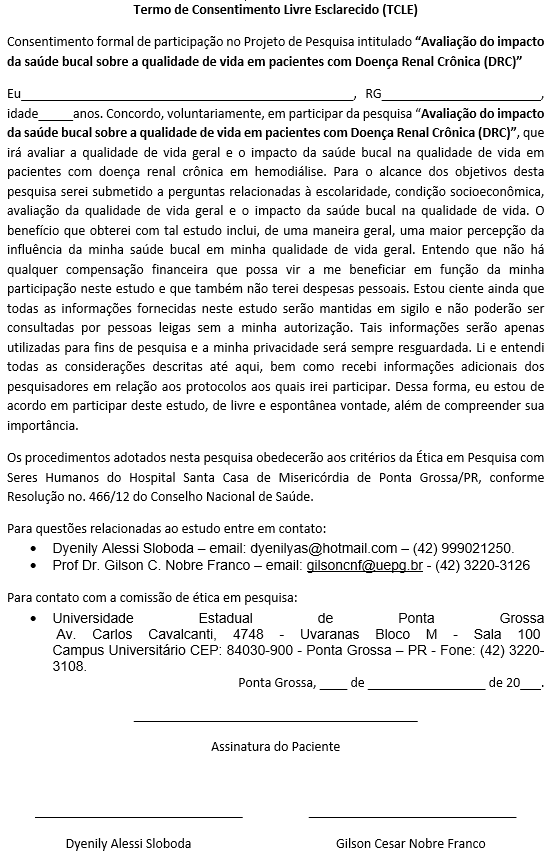
\includegraphics[width=0.62\textwidth]{imagens/anexo1}
\captionsetup{labelformat=empty}
\end{figure}

\end{document}

%%%%%%%%%%%%%%% 
%%%%%%%%%%%%%%% Fim do documento
%%%%%%%%%%%%%%%